\documentclass[bibtotoc,oneside]{scrbook}

\usepackage[a4paper]{geometry}
\usepackage[english]{babel}
\usepackage[utf8]{inputenc}
\usepackage{graphicx}
\usepackage{url}
\usepackage{hyperref}
\usepackage{listings, color}
\usepackage{scrpage2}					% header and footer line
\usepackage{longtable}
\usepackage{subfigure}
\usepackage[nonumberlist, toc]{glossaries}

\usepackage[autostyle]{csquotes}
\usepackage{biblatex}
\nocite{*}

\usepackage{algpseudocode}

\lstset{
    frame=single,
    showspaces=false,
    language=[Objective]Caml
}

\usepackage[nottoc]{tocbibind}

\usepackage{xcolor}
\hypersetup{
    colorlinks,
    linkcolor={red!50!black},
    citecolor={blue!50!black},
    urlcolor={blue!80!black}
}

\usepackage{enumitem}
\usepackage{calc}
\SetLabelAlign{parright}{\parbox[t]{\labelwidth}{\raggedleft#1}}

\usepackage{amssymb}

% header and footer line - no header & footer line on pages where a new chapter starts
\pagestyle{scrheadings}

\graphicspath{{./img/}}

\setacronymstyle{long-short-desc}  % Print both long and short
\renewcommand*{\acronymentry}[1]{%
 \acronymfont{\glsentryshort{#1}} (\textnormal{\glsentrylong{#1}})} % Print it the way I want

\makenoidxglossaries
%!TEX root = ../dokumentation.tex

%
% vorher in Konsole folgendes aufrufen:
%	makeglossaries makeglossaries dokumentation.acn && makeglossaries dokumentation.glo
%

%
% Glossareintraege --> referenz, name, beschreibung
% Aufruf mit \gls{...}
%

%\newacronym{cd}{CD}{compact disk}

\newglossaryentry{Glossareintrag}{name={Glossareintrag},plural={Glossareinträge},description={Ein Glossar beschreibt verschiedenste Dinge in kurzen Worten}}

\newglossaryentry{computer}
{
    name=computer,
        description={is a programmable machine that receives input,
            stores and manipulates data, and provides
                output in a useful format}
}

\newglossaryentry{potato}{name={potato},plural={potatoes},
description={starchy tuber}}
\newglossaryentry{cabbage}{name={cabbage},
description={vegetable with thick green or purple leaves}}
\newglossaryentry{carrot}{name={carrot},
description={orange root}}

%\newacronym{api}{API}{Application Programming Interface }

%%% The glossary entry the acronym links to   
\newglossaryentry{api}{name={API},
    description={An Application Programming Interface (API) is a particular set
    of rules and specifications that a software program can follow to access and
    make use of the services and resources provided by another particular software
    program that implements that API}}

    %%% define the acronym and use the see= option
    %\newglossaryentry{api}{type=\acronymtype, name={API}, description={Application
    %Programming Interface}, first={Application
    %Programming Interface (API)\glsadd{apig}}, see=[Glossary:]{apig}}


\bibliography{./bib/references}

\usepackage{pifont}

\usepackage{afterpage}

\newcommand*\tick{\item[\ding{51}]}
\newcommand*\fail{\item[\ding{55}]}

\newcommand*\pro{\item[$+$]}
\newcommand*\con{\item[$-$]}

\newcommand*\BitAnd{\mathrel{\&}}
\newcommand*\BitOr{\mathrel{|}}
\newcommand*\ShiftLeft{\ll}
\newcommand*\ShiftRight{\gg}
\newcommand*\BitNeg{\ensuremath{\mathord{\sim}}}

\usepackage{tikz}
\usetikzlibrary{positioning}
\usetikzlibrary{shadows,arrows}
\tikzstyle{line} = [draw, thick, color=black!50, -latex']

\definecolor{mybluei}{RGB}{124,156,205}
\definecolor{myblueii}{RGB}{73,121,193}
\definecolor{mygreen}{RGB}{202,217,126}
\definecolor{mypink}{RGB}{233,198,235}

\begin{document}

% ---------------------------------------------------------------
\frontmatter
    \thispagestyle{empty}
\begin{center}

\vspace*{1.4cm}
{\LARGE \textbf{OCaml native debugging}}

\begin{figure}
    \centering
    \subfigure{
\includegraphics[width=60mm]{ocamlpro-logo}}
    \hspace{1em}
    \hfill
    \subfigure{
\includegraphics[width=60mm]{upmc}}
\end{figure}

\vspace*{1.0cm}

{\LARGE Internship Report - Master's Thesis}\\

\vspace{1.0cm}
{\LARGE \textbf{Université Pierre et Marie Curie}}\\
\vspace*{0.3cm}
{\LARGE \textbf{Paris, France}}\\
\vspace*{1.0cm}
{\LARGE Elias BOUTALEB}
\\
\vspace*{0.5cm}
\today
\vspace*{1.0cm}

Supervised by\\
    Jacques MALENFANT (UPMC/LIP6)\\
    Fabrice LEFESSANT (OCamlPro)\\
\vspace*{0.5cm}
\vspace{3cm}


\end{center}


   	\thispagestyle{empty}

    %\thispagestyle{empty}
\vspace*{1.0cm}

\begin{center}
    \textbf{Abstract}
\end{center}

\vspace*{0.5cm}

\noindent
In your thesis you should try to explain as much as possible with the help of images.
\\
\\
The abstract is the most important part of your thesis. Take your time to write it as good as possible. Abstract should have no more than one page. It is normal to rewrite the abstract again and again, so  probaly you won't write the final abstract before the last week of due-date. Before submitting your thesis you should give at least the abstract, the introduction and the conclusion to a native english speaker. It is likely that almost no one will read your thesis as a whole but most people will read the abstract, the introduction and the conclusion.
\\
\\
Start with some introductionary lines, followed by some words why your topic is relevant and why your solution is needed concluding with 'what I have done'. Don't use too many buzzwords. The abstract may also be read by people who are not familiar with your topic.

    %\thispagestyle{empty}
    %\cleardoublepage

    \tableofcontents
    \thispagestyle{empty}

% --------------------------------------------------------------
\mainmatter % comment single chapters for faster compilation
    \chapter{Introduction\label{cha:chapter1}}

There are things to be aware of when dealing with \gls{native}:
\begin{itemize}
    \item it does not retain any information about
        the abstractions of the source programming language in the original
        source code, because the CPU does not need them to run the program,
%backend compiler passes
%reorganize and reposition instructions
    \item compiler \glspl{optim} can move, add and transform code
        in such a way that it might not be possible to identify which
        source code statement corresponds to a particular set of instructions.
\end{itemize}

Hence, compilation of a program to native code involve a huge loss of information,
information that is usually collected by compilers and bundled with binaries and
\glspl{objectfile} in the form of debugging information for debuggers.

\section{Motivation\label{sec:moti}}

There are three main reasons for this work :

\begin{itemize}
    \item Cases where it is necessary to debug native code may arise, e.g a bug
        appearing only in an optimized version of a program.
    \item For now, there is no unified solution for debugging OCaml native
        code on any platform. The bare minimum is here (\gls{backtrace} support,
        partial step by step into function entry points and function calls),
        but mainstream debuggers such as gdb and lldb remain largely unaware that they
        might deal with OCaml native programs.
    \item In that situation, inspecting disassembled code instruction by
        instruction and raw memory becomes a tedious task in a large program,
        that requires knowledge of the target architecture and the OCaml native
        runtime, hence the need for a source-level native debugger.
\end{itemize}

\newpage

\section{Objectives and scope\label{sec:objective}}

The work presented here aims to improve debugging experience concerning OCaml
native compiled code. \\
It involves coordination between the compiler and the debugger:

\begin{itemize}
    \item Modifying the OCaml native compiler to output more debugging
        information, such as line information (mapping between lines in source
        code and machine code addresses) and runtime location of variables, and
        storing that information in a format that a debugger can make
        sense of.
    \item  Improving an OCaml native debugger prototype, written in OCaml and using LLDB
        API bindings, and implementing the main features found in a source-level
        debugger (setting breakpoints, proper symbol handling, stepping into the source
        code, printing values of variables).
\end{itemize}

\section{About OCamlPro}

The OCamlPro company does mainly research and development and provides
consulting services for the purpose of developing and promoting OCaml in the
software development industry.
Notable products/highlights include OCaml online learning tools, contributions
to the Open Source Software community, in particular additions to the OCaml
compiler suite and the SMT solver Alt-Ergo.

%ne consacrez pas plus d’une page
%à la description de l’entreprise et du contexte du stage

%Internship context

%Intern bound to research and development

%Internship timeline (every forthnight)

\section{Outline\label{sec:outline}}

\textbf{Chapter \ref{cha:chapter2}} will give a overview of the DWARF
data debugging format, its structure and show related work around it.
\\
\\
In \textbf{Chapter \ref{cha:chapter3}}, we will have a look at the process of
compilation to native code and additions to that process.
\\
\\
\textbf{Chapter \ref{cha:chapter4}} will tackle the OCaml runtime management of
values will be explained, introduces to LLDB, related binding ocplib-lldb and
the native debugger ocp-lldb.
\\
\\
\textbf{Chapter \ref{cha:chapter5}} will summarize the thesis,
describe/discuss the problems that occurred (issues) and possible future work.

    \chapter{Introduction to the DWARF format\label{cha:chapter2}}

To establish correspondence between high-level source code and low-level machine code, one wants to
\begin{itemize}
    \item  collect all information generated im the compiling process
    \item  and represent that information in a suitable format usable by debuggers, concisely and compactly
\end{itemize}

DWARF is a debugging data format allowing support for source level debugging
it has with the following characteristics:

It is widely used today
it is language agnostic, independent of compiler tooling (linker/assembler),
target architecture and debuggers.
It is somewhat object file agnostic, although mostly associated with the ELF object file format.

it is standardized, meaning it has specifications and norms codified into
a formal document.
A commitee oversees additions/extensions to the standard to follow the
appearance of programming languages and their evolution

\section{Important DWARF sections and their contents}

%\begin{description}[leftmargin=!,labelwidth=\widthof{\bfseries .debug\_abbrev}]
\begin{description}[labelwidth=\widthof{\bfseries .debug\_abbrev},align=parright]
    \item[.debug\_abbrev] Abbreviations used to decode the .debug\_info section
    \item[.debug\_frame] Call frame information table
    \item[.debug\_info] Core DWARF data section
    \item[.debug\_line] Line number information table
    \item[.debug\_loc] Location lists for runtime location of variables/parameters
    \item[.debug\_str] String table reference in .debug\_info
\end{description}

\section{Storage}

The debugging information is stored in sections in the object file.

In the separate compilation process, the DWARF sections of each object file are
put together in their common corresponding section in the final binary

Binary data format

Multiple techniques are used to reduce the size of the debugging information:

LEB128 is a variable length compression encoding
it allows for encoding of signed and unsigned integers of arbitrary size.
Used in DWARF to encode values of various fields (like attributes)

Some of the section tables can become quite large.
In order to save space, those tables are encoded as bytecode instructions to be executed by state machines to obtain their fully expanded form

\section{Structure}

\subsection{Debugging information entry}

In DWARF, the base entity manipulated is called an debugging information entry, or DIE.
A DIE is made of a tag specifying what language construct it describes and a list of attributes giving more details concerning that construct.

A DIE tag can designate for example entities such as:
\begin{description}
    \item[DW\_TAG\_subprogram] — A subroutine/function
    \item[DW\_TAG\_variable] — A variable
    \item[DW\_TAG\_formal\_parameter] — An argument within function parameters
    \item[DW\_TAG\_lexical\_block] - Define lexical scoping of local variables
    \item[DW\_TAG\_base\_type] - Primitive type not defined in terms of other
        types
\end{description}

An attribute is a name/value couple.
The name attribute indicates what the value represents (name, absolute address,
bytecode, offset, string, integer) and what class of values are supported
It is hence possible for attributes values to reference other DIEs and DWARF sections.

\begin{description}
    \item[DW\_AT\_name] String naming the designated DIE
    \item[DW\_AT\_stmt\_list] Offset referencing a location list
    \item[DW\_AT\_type] Reference to a type DIE
    \item[DW\_AT\_low\_pc] address of the first machine instruction
    \item[DW\_AT\_high\_pc] address or offset/constant of the first location past the last instruction
\end{description}

A DIE can be nested in another parent DIE, have siblings and children,
can be represented as a tree with an arbitrary number of children

The subprogram DIE owns DIEs describing the subprogram.

\subsection{Compilation unit}

It designates two entities :

each separately compiled source file is considered as a compilation unit
the root of a DIE tree that starts the DWARF data for the source file it represents
It contains general information about the compilation,
such as the programming language, the compiler version used, source file name, flags

\section{Example}

\section{The ocplib-dwarf library}

Working with DWARF programmatically
it is a library written in OCaml that reads and prints DWARF data in a human readable format similar to objdump
made in a effort to learn and comprehend the DWARF format during the internship.

DWARF emission writing and editing features are not yet implemented
not sure it is useful, as this task is left to compilers

high level desc

%todo prepare a schema

driver with command line option handling

offers abstraction that allow DWARF data manipulation
can visualize the DIE tree structure in debug\_info in DOT format using graphviz
to emulate mutable trees, a zipper library was implemented

utility functions for reading binary data

section parsing implemented accordingly to the DWARF4 standard by its own module
printing module operates on DWARF data structures in ocaml

hexadecimal view available for debugging purposes


    \chapter{The OCaml native compiler\label{cha:chapter3}}

The OCaml language support multiple programming paradigms:

functional programming style, that consists mostly of pure computations that always
evaluate to the same value across different executions for the same arguments
and do not produce side effects.

in contrast, in the imperative programming style
use of assignments to mutable variables can result in side effects
where the return value of a routine may change across multiple executions,
mutate/modifie some state in the program, perform I/O operations
such as reading from/writing to a file

In both styles, stepping through function calls is fine, regardless of whether
they are pure or not.
However, in the case of side-effect functions, one must be vary of the order of
evaluation of arguments, as they may affect the return value.

Moreover, constructs specific to functional programming style such as the map
and filter functions, the use of first class functions taking other functions as
arguments and partial function application/currying,
it may not make much sense to debug this the same way one would with
an imperative language such as C and its equivalent constructs.

\section{Compilation process}

\begin{figure}
  \centering
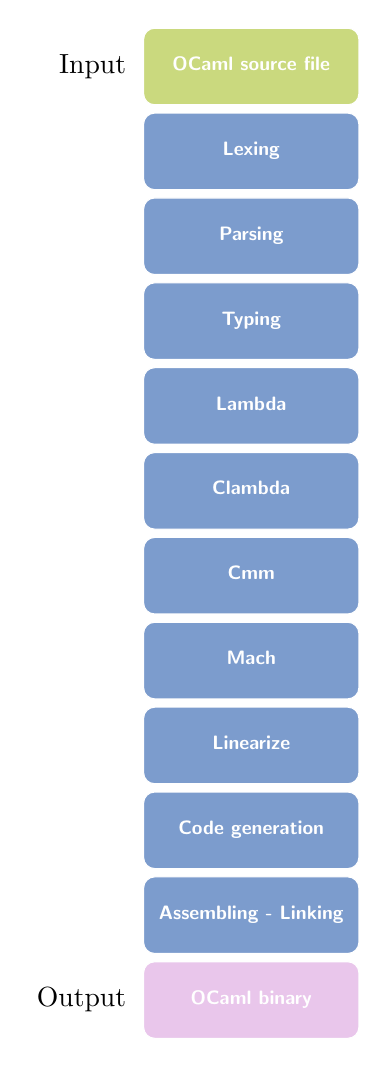
\begin{tikzpicture}[node distance=3pt,outer sep=0pt,
blueb/.style={
  draw=white,
  fill=mybluei,
  rounded corners,
  text width=2.5cm,
  %font=\scriptsize,
  font={\scriptsize\sffamily\bfseries\color{white}},
  align=center,
  text height=12pt,
  text depth=9pt},
greenb/.style={blueb,fill=mygreen},
]
\node[blueb, fill=mygreen] (prog) {OCaml source file};
\node[left=of prog] (i) {Input};
\node[blueb, below=of prog] (lex) {Lexing};
\node[blueb, below=of lex] (par) {Parsing};
\node[blueb, below=of par] (typ) {Typing};
\node[blueb, below=of typ] (lam) {Lambda};
\node[blueb, below=of lam] (clam) {Clambda};
\node[blueb, below=of clam] (cmm) {Cmm};
\node[blueb, below=of cmm] (mac) {Mach};
\node[blueb, below=of mac] (lin) {Linearize};
\node[blueb,below=of lin] (cgen) {Code generation};
\node[blueb,below=of cgen] (asm) {Assembling - Linking};
\node[blueb,fill=mypink,below=of asm] (bin) {OCaml binary};
\node[left=of bin] (o) {Output};
\end{tikzpicture}
\end{figure}

The source program goes through multiple passes/transformations:

\begin{description}
    \item[lexing - lexical analysis]
        split the program from a sequence of characters into a sequence of tokens

    \item[parsetree - syntactic analysis]

        check whether the program as a seq of tokens is gramatically valid, and if so
        construct a base in-memory representation of the program, an abstract syntax
        tree. that AST contains file and line location information.

    \item[typedtree - semantic analysis]
        annotate AST with type information
        type inference and checking

    \item[lambda]
        AST with
        pattern matching optimization,
        % to if and switch constructs,
        elimination of classes and modules,
        discards type information,
        maps the source code to runtime memory model,
        gives unique names to identifiers by append number to them
        (variable shadowing)
        loss of most of location information occurs at this point

    \item[clambda]
        closure conversion, inlining, constant propagation/folding

    \item[cmm]
        primitives conversion, constant folding

    \item[mach]
        register liveness analysis, register allocation

    \item[linearize]
        code as list/seq of pseudo-instructions, close to machine code
        with calls and jumps

    \item[code generation]

    \item[assembling and linking]
\end{description}

Among those steps, all passes up to lambda are common to both bytecode and
native compilers, the ones from clambda onwards are specific to the native compiler

% todo : make figure with all different compilation steps


\section{Additions to the compiler}

Those additions were done and tested on a x86 64-bit system using Linux, on a
closed project fork of the OCaml compiler, including memory profiling
facilities.

\subsection{Location information}

Let us define first what a debugging event is, quoting the OCaml manual:

\begin{quotation}
    Events are “interesting” locations in the source code, corresponding to the
    beginning or end of evaluation of “interesting” sub-expressions. Events are
    the unit of single-stepping (stepping goes to the next or previous event
    encountered in the program execution). Also, breakpoints can only be set at
    events. Thus, events play the role of line numbers in debuggers for
    conventional languages. \autocite{events}
\end{quotation}

Those events are here used in the bytecode with the bytecode, source-level
debugger \textit{ocamldebug}. \\

Among the debugging information to be added, line information is important,
both for stepping into the source program statement by statement,
and also for setting breakpoints by file and line number.

The idea here is to propagate the location information contained in those events
through the native code backend, by wrapping all AST/IR nodes into a record
containing the node and a field with location information from the debugging
event.

\begin{lstlisting}
type t = {
  dinfo_file: string;
  dinfo_line: int;
  dinfo_char_start: int;
  dinfo_char_end: int
}

type 'a expression = {
  exp: 'a;
  dbg: t;
}
\end{lstlisting}

This has been done for every native backend pass all the way up to the linearize
pass, whose instruction record that already contains such a field.

At the code generation step, the code emitter uses two notable debugging
assembly directives, specific to the GNU assembler as it is used in the
compilation process:

%https://sourceware.org/binutils/docs-2.26/as/Loc.html
%https://sourceware.org/binutils/docs-2.26/as/File.html

\begin{itemize}
    \item .file fileno filename : assigning a positive integer to a filename
    \item .loc fileno lineno [column] [options] : add a row to the .debug\_line
        line information matrix for the current compilation unit, map a source
        file and line number to the assembly instructions that follow

\end{itemize}

% dans le code assembleur, présence de directives .loc
%fichier - num de ligne - num de colonne
%assembleur recupere les infos et l'offset et encode tout cela dans une structure dediée dans la section .debug\_line

Then/afterwards, location information was attached to some particular nodes/constructs

integers - as empty list [] and None from the option type represented as integers
primitives - explain what a primitive is, what it is responsible for

prim operations mirroring bytecode instructions maybe?
may refer to external C function
assignments, allocation, comparisons, /string/float/integer/boolean operations,
boxed/unboxed

setfield primitive - responsible for mutable assignments

\begin{description}
\pro more info
\con less precision
\end{description}

\begin{itemize}
\tick more info
\fail less precision
\end{itemize}

Heavy modifications on the backend
% huge patch when trying to add a debugging field to every IR node
% languages des passes backend natif n'a pas prevu pour l'adjonction d'info de debug
lack of accuracy, loss of information still occuring as code is still expanded and transformed
%\item Valeurs disponibles pas toujours cohérentes
% csq du manque de precision
as a csq of lack of precision, location information directives arent put at the
most suitable assembly instruction, values might not be updated when they should
and vice versa

\subsection{Runtime location of variables}


Add 2 passes into the backend: available\_regs and available\_ranges
using forward data-flow analysis operating on Mach IR, can be traversed like
a CFG

% https://stackoverflow.com/questions/11322163/ocaml-calling-convention-is-this-an-accurate-summary

ocaml calling conventions different from C, where arguments are passed in
registers, ocaml runtime tries to reuse registers as much as it can, variables
spilled on the stack if no registers available
callees are free to destroy their callers' arguments

available\_regs
takes a function expressed in Mach code as input
return Mach code with each ins annotated with set of `registers` identifiers
whose value can be accessed (hence available) by a debugger at runtime

The data-flow equations used for a given instruction
\[
    \textit{out}_{b} = \bigcup_{s \in succ_{b}} \textit{in}_{s}
\]
\[
    \textit{in}_{b} = (\textit{out}_{b} - \textit{kill}_{b}) \cup \textit{gen}_{b}
\]

%out(b) = 0
%for s in succ(b)
  %out(b) = out(b) or in(s)
  %in(b) = (out(b) and not kill(b)) or gen(b)
available\_ranges:
operates over available\_regs output as input
calculates for each variable/ identifier used in target function the memory
addresses ranges where its content can be inspected, and for each range, the
place where the content can be accessed (in registers or on the stack)

\begin{algorithmic}[1]
    \If{some condition is true}
    \State do some processing
    \ElsIf{some other condition is true}
    \State do some different processing
    \ElsIf{some even more bizarre condition is met}
    \State do something else
    \Else
    \State do the default actions
    \EndIf
\end{algorithmic}

populate the  .debug\_info et .debug\_loc sections

unique identifier with unique stamp is generated in cases variable shadowing overwrites former value

not every value binding is captured becaused of constant folding


for each, what effect is achieved, tradeoffs
what/why/how

\subsection{DWARF emitter}

for each, what effect is achieved, tradeoffs
what/why/how

\subsection{Type information}


typed AST is serialized into the binary instead of a separate file

more practical to manipulate, comes at the cost of a bigger binary size

representation will be used later to build a symbol table for use in ocp-lldb


for each, what effect is achieved, tradeoffs
what/why/how


    TODO:
We developed the first prototype of a native debugger for OCaml, based on the LLDB debugging framework on top of LLVM. For that, we first generated a full OCaml binding for the LLDB library, by parsing the C++ headers of the libraries and automatically generating OCaml and C++ stubs. We were then able to use the OCaml binding to develop several tools, ranging from a simple tool that displays the internal GC information of a finished OCaml application, to an almost complete debugger, which displays OCaml values using runtime type information added for memory profiling.


\chapter{Concept\label{cha:chapter4}}
This chapter introduces the architectural design of Component X. The component consists of subcomponent A, B and C.

In the end of this chapter you should write a specification for your solution, including interfaces, protocols and parameters.

\section{Sub-component A\label{sec:conceptsuba}}
The concept chapter provides a high-level explanation of your solution. Try to explain the overall structure with a picture. You can also use UML sequence diagrams for explanation.

Figure \ref{fig:aliceandbob} illustrates the situation between Alice and Bob. (sequence diagram from www.websequencediagrams.com)

\begin{figure}[htb]
  \centering
  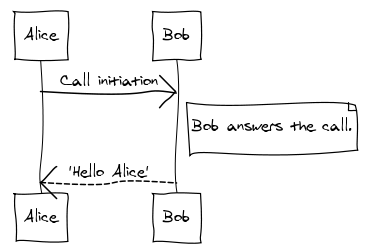
\includegraphics[width=9cm]{uml_seq_example.png}\\
  \caption{Alice and Bob}
  \label{fig:aliceandbob}
\end{figure}

\section{Sub-component B\label{sec:conceptsubb}}

Lorem Ipsum...

\section{Proposed API\label{sec:conceptsubb}}

Lorem Ipsum...

\section{Layer X\label{sec:conceptlayerx}}

Lorem Ipsum...

\section{Interworking of X and Y\label{sec:conceptinter}}

Lorem Ipsum...

\section{Interface Specification\label{sec:intspec}}

Lorem Ipsum...


    \chapter{Evaluation\label{cha:chapter5}}

In this chapter the implementation of Component X is evaluated. An example instance was created for every service. The following chapter validates the component implemented in the previous chapter against the requirements.
\\
\\
Put some screenshots in this section! Map the requirements with your proposed solution. Compare it with related work. Why is your solution better than a concurrent approach from another organization?

\section{Test Environment\label{sec:testenvir}}

Fraunhofer Institute FOKUS' Open IMS Playground was used as a test environment for the telecommunication services. The IMS Playground ...

\section{Scalability\label{sec:scal}}

Lorem Ipsum

\section{Usability\label{sec:usab}}

Lorem Ipsum

\section{Performance Measurements\label{sec:performance}}

Lorem Ipsum

% ---------------------------------------------------------------
\backmatter
    \printnoidxglossaries

\endinput

    \addchap{Annex}

\begin{appendix}

\lstset{
    numbers=left,
    basicstyle=\ttfamily\footnotesize,
    frame=single, % adds a frame around the code
    xleftmargin=3.4pt,
    xrightmargin=3.4pt
}

\lstinputlisting[caption=C program example,language=C, label={lst:tc}]{./t.c}

\begin{minipage}{\linewidth}
\lstinputlisting[firstline=22, lastline=51, label={lst:asm}, caption=x86\_64 assembly output of example program from line 4 to 11]{./t_ex.s}
\end{minipage}

\newpage

\begin{minipage}{\linewidth}
\lstinputlisting[lastline=52, caption=Output of .debug\_info section decoding from example program]{./t.dwarf}
\end{minipage}

\newpage

\begin{minipage}{\linewidth}
\lstinputlisting[firstline=53, firstnumber=53, label={lst:dwa}]{./t.dwarf}
\end{minipage}

\end{appendix}

\endinput

    \printbibliography

\end{document}
